\RequirePackage{luatex85}
\documentclass{standalone}

% Default preamble
\usepackage{pgfplots}
\usepackage{tikz}
\pgfplotsset{compat=newest}
\usepgfplotslibrary{groupplots}
\usepgfplotslibrary{polar}
\usepgfplotslibrary{smithchart}
\usepgfplotslibrary{statistics}
\usepgfplotslibrary{dateplot}
\usepgfplotslibrary{ternary}

% Custom preamble from global variable:
\usetikzlibrary{patterns}
\usepackage{xcolor}
\definecolor{cred}{HTML}{ED1C24}
\definecolor{cgrey}{HTML}{7F7F7F}
\definecolor{cblue}{HTML}{00A2E8}
\definecolor{cgreen}{HTML}{22B14C}
\definecolor{cyellow}{HTML}{FFF200}
\definecolor{corange}{HTML}{EA7904}
\definecolor{cpurple}{HTML}{9100FC}
\definecolor{julia1}{HTML}{1F77B4}
\definecolor{julia2}{HTML}{FF7F0E}
\definecolor{julia3}{HTML}{2CA02C}

\usepackage{caption}
\usepackage{subcaption}
\usepackage{amsmath}

\renewcommand{\familydefault}{\sfdefault}

\begin{document}

    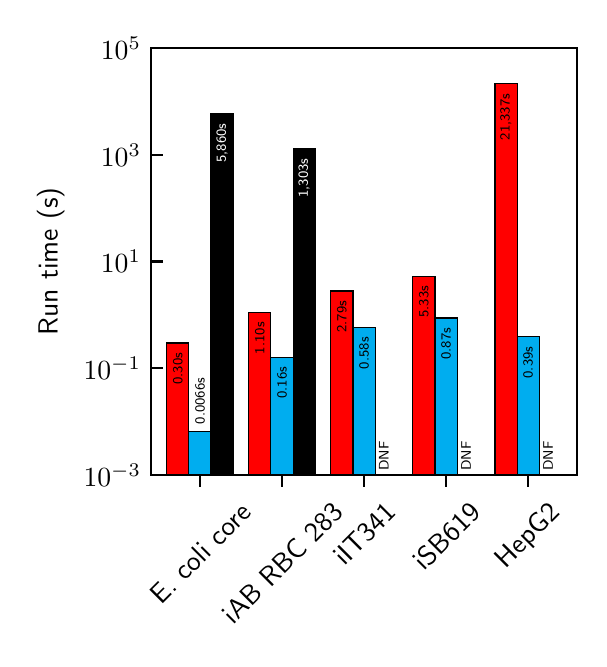
\begin{tikzpicture}
        \begin{axis}[%
            height=7cm,
            width=7cm,
            ybar  = 0pt,
            ymode = log,
            xmajorgrids={false},
            ymajorgrids={false},
            xtick pos = bottom,
            ytick pos = left,
            bar width = 8pt,
            legend image code/.code={\draw [#1] (0cm,-0.1cm) rectangle (0.2cm,0.25cm);},
            legend cell align={left}, 
            legend style={%
                at={(-0.285,-0.2)},
                anchor={north},
                legend columns={1},
                thick,
            },
            ylabel={Run time (s)},
            ymin={1},
            ymax={100000000},
            ytick={1,100,10000,1000000, 100000000},
            yticklabels={{$10^{-3}$}, {$10^{-1}$}, {$10^{1}$}, {$10^{3}$}, {$10^{5}$}},
            xmin={0.4},
            xmax={5.6},
            xtick={1,2,3,4,5},
            xticklabels={%
                {E. coli core},
                {iAB RBC 283},
                {iIT341},
                {iSB619},
                {HepG2},
            },
            x tick label style={rotate=45},
            axis line style={thick,black},
            minor tick style={draw=none},
            xtick style={/pgfplots/on layer=axis foreground, thick, black},
            ytick style={/pgfplots/on layer=axis foreground, thick, black},
            legend to name=leg2,
        ]
            \addplot[black, fill=red] % Julia MarkovWeightedEFMs.jl (carbon)
                coordinates {
                    (1,296.12612724304200)
                    (2,1101.1159420013428)
                    (3,2789.4294261932373)
                    (4,5327.3885250091550)
                    (5,21337208.898544310)
                };
            \addplot[black, fill=cyan] % Julia MarkovWeightedEFMs (nitrogen)
                coordinates {
                    (1,006.600856781005859)
                    (2,160.629510879516600)
                    (3,578.065395355224600)
                    (4,870.053291320800800)
                    (5,386.489868164062500)
                };
            \addplot[black, fill=black] % MATLAB FluxModeCalculator (serial)
                coordinates {
                    (1,5859564.1)
                    (2,1303479.5)
                    (3,1.0001)
                    (4,1.0001)
                    (5,1.0001)
                };

            % E coli core bars
            \node [left,font=\tiny,anchor=east,rotate=90] at (axis cs: 0.73,296) {0.30s};
            \node [right,font=\tiny,anchor=east,rotate=90] at (axis cs: 1,100.6) {0.0066s};
            \node [right,font=\tiny,anchor=east,rotate=90,white] at (axis cs: 1.27,5858564.1) {5,860s};
           
            % iAB RBC 283 bars
            \node [right,font=\tiny,anchor=east,rotate=90] at (axis cs: 1.73,1101) {1.10s};
            \node [right,font=\tiny,anchor=east,rotate=90] at (axis cs: 2,160.6) {0.16s};
            \node [right,font=\tiny,anchor=east,rotate=90,white] at (axis cs: 2.27,1303479.5) {1,303s};

            % iIT341 bars
            \node [right,font=\tiny,anchor=east,rotate=90] at (axis cs: 2.73,2789.4) {2.79s};
            \node [right,font=\tiny,anchor=east,rotate=90] at (axis cs: 3,578.0) {0.58s};
            \node [above,font=\tiny,rotate=90] at (axis cs: 3.42,2.25) {DNF};

            % iSB619 bars
            \node [right,font=\tiny,anchor=east,rotate=90] at (axis cs: 3.73,5327.4) {5.33s};
            \node [right,font=\tiny,anchor=east,rotate=90] at (axis cs: 4,870.0) {0.87s};
            \node [above,font=\tiny,rotate=90] at (axis cs: 4.42,2.25) {DNF};

            % HepG2 bars
            \node [right,font=\tiny,anchor=east,rotate=90] at (axis cs: 4.73,21337208.9) {21,337s};
            \node [right,font=\tiny,anchor=east,rotate=90] at (axis cs: 5,386.5) {0.39s};
            \node [above,font=\tiny,rotate=90] at (axis cs: 5.42,2.25) {DNF};

            \legend{{MarkovWeightedEFMs.jl (serial)}, {MarkovWeightedEFMs.jl (serial)}, {FluxModeCalculator (serial)}}
        \end{axis}
    \end{tikzpicture}

\end{document}

